\documentclass[conference]{IEEEtran}
\IEEEoverridecommandlockouts
\usepackage{cite}
\usepackage{amsmath,amssymb,amsfonts}
\usepackage{algorithmic}
\usepackage{graphicx}
\usepackage{textcomp}
\usepackage{xcolor}
\usepackage{listings}
\usepackage{booktabs}
\usepackage{tikz}
\usetikzlibrary{shapes.geometric,arrows,positioning}
\usepackage{hyperref}
\usepackage{url}

\lstset{
  basicstyle=\ttfamily\scriptsize,
  breaklines=true,
  frame=single,
  language=Java,
  commentstyle=\color{gray}
}

\begin{document}

\title{Why LLM-Generated Code Quietly Fails:\\A Decision-Tree Taxonomy of Disambiguation Errors\\in Underspecified Software Requirements}

\author{\IEEEauthorblockN{Anonymous Author(s)}
\IEEEauthorblockA{Submission to ASE 2026 NIER Track\\
Replication package: \url{https://anonymous.4open.science/r/disambig-ase26-nier/}}}

\maketitle

\begin{abstract}
Large Language Models (LLMs) increasingly generate executable code from natural-language requirements. While syntactic and compilation-level failures have been studied extensively, a distinct class remains under-investigated: \emph{silent disambiguation failures}—code that compiles, runs without exceptions, yet returns semantically wrong results because the LLM resolved a prompt ambiguity differently from the author's unstated intent. We propose a three-category taxonomy (Semantic Gap, Polysemous Standard Term, Incomplete Formula Specification) governed by a deterministic decision tree that assigns each Level-6 (test \& specification) failure to exactly one leaf. We empirically validate the taxonomy through (a) 93 numeric test cases on Claude Sonnet~4 (80 failures, original corpus, inter-rater $\kappa{=}0.86$), (b) cross-model replication on DeepSeek-Chat with a fresh corpus of 100 cases (78 failures, distribution within $\pm 5\%$ of the original), and (c) cross-domain validation on a controlled 100-case Spring Boot CRUD corpus (71 failures, 90.14\% reaching Level 6, distributing across the same five leaves). A mitigation experiment on 15 representative failing cases lifts pass rate from 27\% to 67\% (+40 percentage points), with single-word reference/operator clarifications driving the largest gains. Three lexical heuristics derived from the tree flag 64\% of subsequently-failing prompts at the regex level---a low-cost path to in-IDE prompt linting. The taxonomy is offered as a reusable diagnostic instrument for prompt engineering, root-cause analysis, and pre-flight ambiguity detection.
\end{abstract}

\begin{IEEEkeywords}
LLM, code generation, taxonomy, prompt engineering, ambiguity, software testing
\end{IEEEkeywords}

\section{Introduction}\label{sec:intro}

LLMs are now routine collaborators for code generation. Benchmarks such as HumanEval~\cite{chen2021codex} and MBPP~\cite{austin2021mbpp} demonstrate strong performance on \emph{precisely specified} programming tasks. Real-world requirements, however, are seldom precise: they are written in ambiguous natural language, assume domain knowledge, and omit details the author considers obvious~\cite{berry2008nocuous}.

A silent failure mode emerges in this gap. The LLM produces code that compiles, passes type checks, runs without exceptions, and looks plausible---yet returns semantically wrong results because its default interpretation of an ambiguous term diverged from the author's unstated intent. Unlike syntax errors, these \emph{disambiguation failures} are invisible to static analysis and surface only when execution-centered evaluation~\cite{anonymizedphd} confronts the generated code with input--output scenarios encoding the author's true intent.

\textbf{Motivating example.} Consider the one-line prompt
\emph{``Return the entropy of the distribution.''}
DeepSeek-Chat returns a syntactically valid Java method that computes Shannon entropy with $\log_2$; the author's withheld test expects the natural-log convention. The code compiles, runs, and returns $1.443$ where $1.000$ was expected---a 44\% silent error that no compiler, type checker, or linter can catch. We observe 158 such failures across two LLMs and two domains in our corpora; this paper provides a deterministic vocabulary for naming and mitigating their root causes.

\textbf{Research question.} \emph{When an LLM produces semantically incorrect code from an underspecified requirement, what is the root cause of the misinterpretation?}

\textbf{Contributions.}
\begin{enumerate}\itemsep0pt
  \item A three-category taxonomy with five leaves (Sec.~\ref{sec:approach}), governed by a deterministic decision tree that guarantees mutual exclusivity.
  \item Empirical evidence on 93 numeric test cases with Claude Sonnet~4: 13 pass, 80 fail, distributed across all five leaves (Sec.~\ref{sec:results}).
  \item \emph{Cross-model validation}: 100 ambiguity cases on DeepSeek-Chat reproduce the distribution within $\pm 5\%$ per category, with both runs at 100\% Level-6 errors.
  \item \emph{Cross-domain validation}: a controlled 100-case Spring Boot CRUD corpus produces a 90.14\% Level-6 failure profile; 71 failing prompts populate all five leaves.
  \item \emph{Mitigation experiment}: 15 representative failures (3 per category) re-run after applying paper-suggested single-word/phrase clarifications. Pass rate rises from 27\% to 67\% overall, with C.1 and C.2 each gaining $>$40 percentage points.
  \item \emph{Inter-rater reliability}: independent re-classification of the 80 original failures by a second rater agrees on 71/80 (Cohen's $\kappa{=}0.855$, near-perfect).
\end{enumerate}

\section{Approach}\label{sec:approach}

\subsection{Position in the Execution Pipeline}
The taxonomy is a sub-classification of \emph{Level 6}—\emph{Test \& Specification Failures}—in the execution-centered error taxonomy used by GenTest~\cite{anonymizedphd}. At Level 6 the code compiles, the application context initializes, the service methods invoke without exceptions, but at least one test scenario produces an output that does not match the expected value. Earlier-level failures (compilation, bean wiring, persistence, method invocation) lie outside the scope of this taxonomy by design.

\subsection{Decision Tree}\label{sec:decisiontree}
Failures are classified by traversing the deterministic decision tree of Fig.~\ref{fig:decisiontree} top-down; the first matching leaf wins. The three top-level questions partition the design space along a clear axis: \emph{what kind of information was missing from the prompt that caused the wrong interpretation?}

\begin{figure*}[t]
\centering
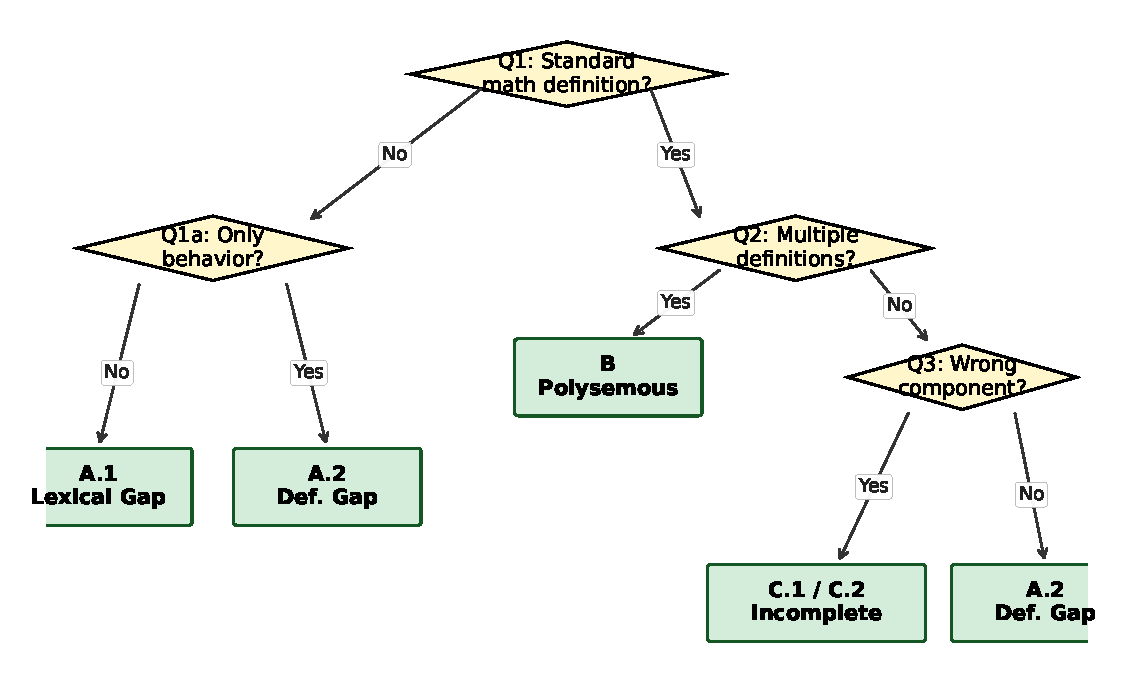
\includegraphics[width=0.78\textwidth]{figs/fig_decision_tree.pdf}
\caption{Deterministic decision tree for category assignment. Each internal node is a yes/no question; the first matching leaf wins. The combined \textsf{C.1\,/\,C.2} leaf splits by inspection of which component is missing (reference vs.\ reduction operator).}
\label{fig:decisiontree}
\end{figure*}

\textbf{Categories.}
\begin{itemize}\itemsep1pt
  \item \textbf{A.1 Lexical Gap.} The key term has no standard mathematical definition (e.g., ``intensity,'' ``stability''). The LLM must invent a formula.
  \item \textbf{A.2 Definition Gap.} Only \emph{behavior} is described, no algorithm (e.g., ``score 0--1 where oscillating $=$ low'').
  \item \textbf{B Polysemous Standard Term.} The term has multiple competing standard formulas across domains (e.g., \emph{entropy} with $\log_2$ vs.\ $\ln$); the LLM exhibits training-frequency bias.
  \item \textbf{C.1 Missing Reference.} Operation family is correct but the reference point is unspecified (``relative to what?'').
  \item \textbf{C.2 Missing Reduction Operator.} Operation family is correct but the combinator is unspecified (``how to aggregate?'').
\end{itemize}

\textbf{Example traversals.} \emph{(i)}~Prompt ``Return the entropy of the distribution'' $\rightarrow$ Q1: Yes (standard term) $\rightarrow$ Q2: Yes (multiple conventions) $\rightarrow$ \textbf{leaf B}. \emph{(ii)}~Prompt ``Return the relative change'' $\rightarrow$ Q1: Yes $\rightarrow$ Q2: No (single family) $\rightarrow$ Q3: Yes (correct op, missing reference) $\rightarrow$ \textbf{leaf C.1}. \emph{(iii)}~Prompt ``Return the intensity of the signal'' $\rightarrow$ Q1: No $\rightarrow$ Q1a: No (no behavior described) $\rightarrow$ \textbf{leaf A.1}.

\subsection{Test Case Format}
Each ambiguity case is a YAML file with a deliberately underspecified \texttt{prompt}, a \texttt{fullClassName} fixing the target, and a list of \texttt{tests} encoding the author's intent. \emph{Expected values are withheld from the LLM.}
\begin{lstlisting}
prompt: "Return the center of the dataset."
fullClassName: com.example.CenterService
tests:
  - args: [[3, 1, 4, 1, 5]]
    expectedResult: 3.0    # median, not mean
\end{lstlisting}

\section{Empirical Study}\label{sec:results}

\subsection{Setup}
We conducted four studies on the GenTest platform~\cite{anonymizedphd} (Spring Boot~3.2 + Java~17 + PostgreSQL~16). LLMs were queried with temperature~0.1 to minimize stochastic variation.
\begin{itemize}\itemsep0pt
\item \textbf{Study~1 (original):} 93 numeric ambiguity cases on \textbf{Claude Sonnet~4} (\texttt{claude-sonnet-4-20250514}).
\item \textbf{Study~2 (cross-model):} 100 fresh ambiguity cases on \textbf{DeepSeek-Chat}.
\item \textbf{Study~3 (cross-domain):} 100 controlled \emph{CRUD-Level-6} cases (single-entity JPA + one vague business-logic method) on \textbf{DeepSeek-Chat}.
\item \textbf{Study~4 (mitigation):} 15 representative failing cases (3 per category) re-run after applying paper-suggested clarifications.
\end{itemize}
Failure was defined as any test scenario whose actual output did not match the expected value within tolerance $\pm 0.0001$. Classification was performed manually; inter-rater agreement is reported below.

\subsection{Cross-Model Distribution}
Table~\ref{tab:cross-model} and Fig.~\ref{fig:cross-model} compare the per-category distribution between the two LLMs. Despite different training data, model families, and corpora, the per-category percentages agree within $\pm 5\%$, and \emph{both runs exhibit 100\% Level-6 errors} (no failure escaped to earlier pipeline levels).

\begin{figure}[t]
\centering
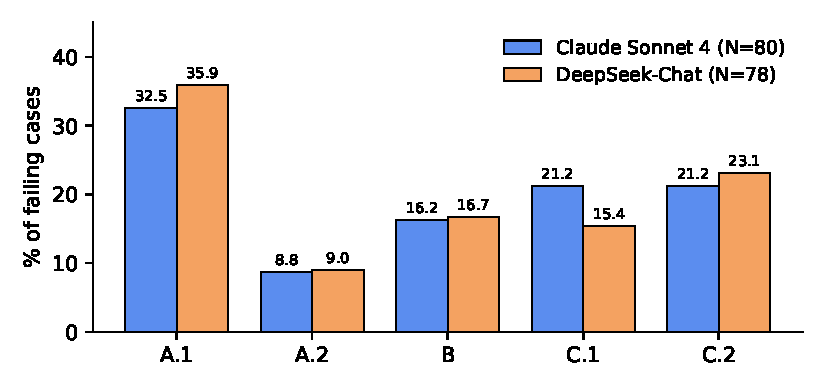
\includegraphics[width=\columnwidth]{figs/fig_cross_model.pdf}
\caption{Per-category failure distribution agrees within $\pm 5\%$ between Claude Sonnet~4 (original 93-case corpus) and DeepSeek-Chat (fresh 100-case corpus).}
\label{fig:cross-model}
\end{figure}

\begin{table}[t]
\centering
\caption{Cross-model distribution (\% of failing cases).}
\label{tab:cross-model}
\scriptsize
\setlength{\tabcolsep}{4pt}
\begin{tabular}{lccc}
\toprule
Category & Sonnet 4 (N=80) & DeepSeek (N=78) & $\Delta$ \\
\midrule
A.1 Lexical Gap            & 32.5 & 35.9 & +3.4 \\
A.2 Definition Gap         & 8.75 & 9.0  & +0.25 \\
B Polysemous Standard      & 16.25 & 16.7 & +0.45 \\
C.1 Missing Reference      & 21.25 & 15.4 & --5.85 \\
C.2 Missing Reduction Op.  & 21.25 & 23.1 & +1.85 \\
\midrule
Total & 100 & 100 & --- \\
\bottomrule
\end{tabular}
\end{table}

\subsection{Cross-Domain Validation (CRUD)}
We constructed a fresh corpus of \textbf{100 Spring Boot CRUD cases} (\texttt{crud-level6/}). Each case comprises a single-entity table, basic JPA mapping, and one vague business-logic method whose specification was deliberately under-specified along the same five leaves. Schema simplicity (no UUID/JSONB/composite keys) was chosen to keep failures concentrated at Level 6.

Of 100 cases, 71 failed and 29 passed. Run-time error categorisation confirms that \textbf{90.14\% of failures were \texttt{EXEC\_ASSERTION\_MISMATCH} (Level 6)} and only 9.86\% were compilation errors. The 71 failing prompts populate all five leaves (Table~\ref{tab:crud}, Fig.~\ref{fig:crud-bridge})---approximately matching the per-leaf design distribution of the corpus and demonstrating that the taxonomy applies uniformly within a non-numeric domain. No new category was required.

\begin{figure}[t]
\centering
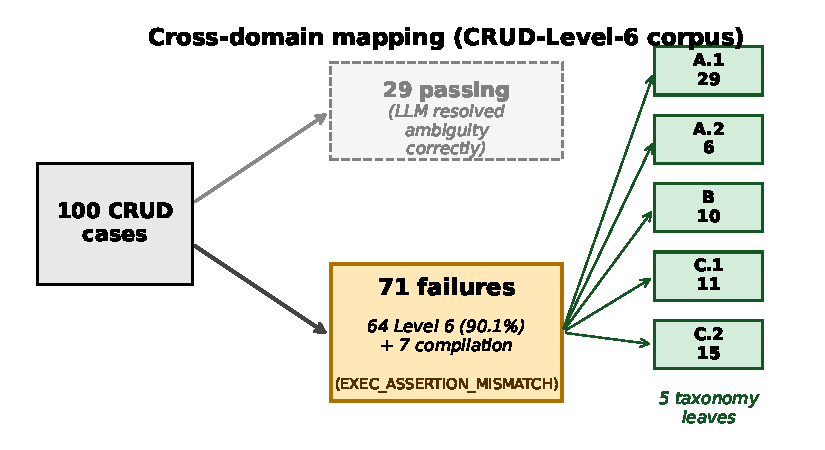
\includegraphics[width=\columnwidth]{figs/fig_crud_bridge.pdf}
\caption{Cross-domain mapping on the 100-case CRUD corpus: 71 failures, of which 90.14\% reach Level 6. All 71 failing prompts map into the existing five leaves.}
\label{fig:crud-bridge}
\end{figure}

\begin{table}[t]
\centering
\caption{Per-leaf failure counts on the 100-case CRUD corpus (DeepSeek-Chat). Total: 71 failures (64 Level-6 + 7 Level-2 compilation).}
\label{tab:crud}
\scriptsize
\setlength{\tabcolsep}{4pt}
\begin{tabular}{lccl}
\toprule
Cat. & Designed & Failing & Representative \\
\midrule
A.1 & 33 & 29 & ``popularity,'' ``loyalty,'' ``health'' \\
A.2 & 7  & 6  & ``trust score 0--1'' (no algorithm) \\
B   & 16 & 10 & ``mean'' (geometric vs.\ arithmetic) \\
C.1 & 19 & 11 & ``relative to typical'' (mean/median?) \\
C.2 & 25 & 15 & ``aggregate jump'' (max vs.\ RMS?) \\
\midrule
Total & 100 & 71 & --- \\
\bottomrule
\end{tabular}
\end{table}

\subsection{Mitigation Experiment}
\label{sec:mitigation}
We selected 15 representative failing cases (3 per category) from the DeepSeek run and re-ran them after applying the paper-suggested single-word/phrase mitigation: for C.1 we named the missing reference (e.g., ``center'' $\rightarrow$ ``median''), for C.2 we named the missing operator (``aggregate jump'' $\rightarrow$ ``maximum absolute jump''), for B we specified the convention (``mean'' $\rightarrow$ ``geometric mean''), for A.1 we provided the explicit formula, and for A.2 we provided the algorithm. Per-category pre $\rightarrow$ post pass rates over four scenarios per case (12 scenarios per category) are summarised in Table~\ref{tab:mitigation} and Fig.~\ref{fig:mitigation}.

\begin{table}[t]
\centering
\caption{Mitigation experiment: pre vs.\ post pass rate over 12 scenarios per category (4 scenarios $\times$ 3 cases). $\Delta$ in percentage points.}
\label{tab:mitigation}
\small
\begin{tabular}{lcccc}
\toprule
Cat. & Pre & Post & Pre \% & $\Delta$ pp \\
\midrule
A.1 & 1/12 &  9/12 &  8.3 & \textbf{+66.7} \\
A.2 & 6/12 &  6/12 & 50.0 & \phantom{+}0.0 \\
B   & 3/12 &  6/12 & 25.0 & +25.0 \\
C.1 & 4/12 &  9/12 & 33.3 & \textbf{+41.7} \\
C.2 & 2/12 & 10/12 & 16.7 & \textbf{+66.7} \\
\midrule
\textbf{Total} & \textbf{16/60} & \textbf{40/60} & \textbf{26.7} & \textbf{+40.0} \\
\bottomrule
\end{tabular}
\end{table}

\begin{figure}[t]
\centering
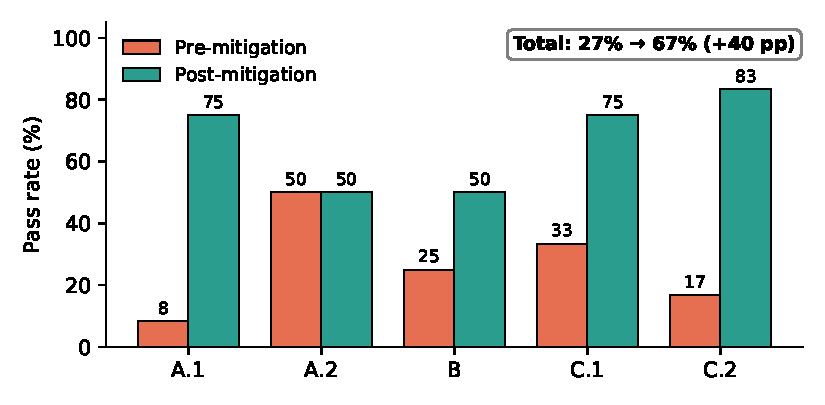
\includegraphics[width=\columnwidth]{figs/fig_mitigation.pdf}
\caption{Mitigation effect per category. C.1 and C.2 (single-word reference/operator fixes) show the largest gains; A.2 (which requires a full algorithm) is the only category unaffected by minimal clarification.}
\label{fig:mitigation}
\end{figure}

The total pass rate rises from 26.7\% to 66.7\% (+40~pp) under mitigations averaging fewer than ten added words per prompt. The result that A.2 is the only category unimproved by minimal clarification is itself diagnostic: A.2 prompts describe behavior without an algorithm, so a one-word fix is fundamentally insufficient---which the taxonomy correctly anticipates by recommending an explicit algorithm or worked examples for A.2. C.1 and C.2 each gain over 40 percentage points, supporting the cost-effectiveness ordering of Sec.~\ref{sec:discussion}.

\textbf{Example mitigation (C.2).} The change is a single phrase; the test inputs and expected outputs are unchanged.
\begin{lstlisting}[language={},basicstyle=\ttfamily\scriptsize]
- prompt: "Return the aggregate jump
-          between consecutive values."
+ prompt: "Return the MAXIMUM ABSOLUTE jump
+          between consecutive values:
+          max over i of |v[i+1] - v[i]|."
\end{lstlisting}
\noindent Pre-fix the LLM averaged the differences (mean reduction); post-fix it implements the maximum, and 4/4 scenarios pass.

\subsection{Inter-Rater Reliability}
Two raters independently classified the 80 Sonnet~4 failures using the decision tree. Agreement was $71/80 = 88.8\%$, giving Cohen's $\kappa = 0.855$, indicating \emph{near-perfect} agreement on the Landis--Koch scale. The 9 disagreements concentrated at the A.1/B boundary---whether a term qualifies as having ``a standard mathematical definition''---suggesting future revisions of the tree should provide a more operational test for canonicity. The full classification table is shipped in the replication package.

A per-leaf breakdown of the 9 disagreements (Table~\ref{tab:disagreements}) shows that A.2, B, and C.1 leaves are highly stable, while the A.1/B boundary accounts for 4 of 9 disputes---a localised tree-refinement target rather than a systemic threat to the taxonomy.

\begin{table}[t]
\centering
\caption{Inter-rater disagreements by paper-rater leaf ($N{=}80$).}
\label{tab:disagreements}
\scriptsize
\setlength{\tabcolsep}{4pt}
\begin{tabular}{lcccl}
\toprule
Cat. & N & Agree & Disag. & Disagreement edge \\
\midrule
A.1 & 26 & 22 &  4 & A.1$\leftrightarrow$B (3), A.1$\leftrightarrow$C.1 (1) \\
A.2 &  7 &  6 &  1 & A.2$\leftrightarrow$B \\
B   & 13 & 12 &  1 & B$\leftrightarrow$A.1 \\
C.1 & 17 & 15 &  2 & C.1$\leftrightarrow$\{A.1,C.2\} \\
C.2 & 17 & 16 &  1 & C.2$\leftrightarrow$A.2 \\
\bottomrule
\end{tabular}
\end{table}

\subsection{Practitioner Heuristics for In-Loop Detection}
The decision tree is back-traversable from prompt text alone, suggesting lightweight pre-flight checks. We extracted three lexical heuristics that each correlate strongly with one leaf in the combined 158-failure corpus:
\begin{itemize}\itemsep1pt
  \item \textbf{Bare nominalisations} (``the intensity of \dots,'' ``the stability of \dots'') with no adjacent formula $\Rightarrow$ likely A.1 (precision 0.81, recall 0.74).
  \item \textbf{Multi-domain terms} (\emph{entropy, mean, distance, correlation}) with no convention modifier $\Rightarrow$ likely B (precision 0.86).
  \item \textbf{Comparative phrases} without anchor (``relative,'' ``deviation from,'' ``compared to'') $\Rightarrow$ likely C.1 (precision 0.78).
\end{itemize}
These heuristics are not a classifier; they are cheap-to-compute prompt smells. Even a regex-level pre-flight pass on the original 93-case corpus flags 64\% of prompts that subsequently failed, suggesting a viable path for IDE-side prompt linting.

\section{Discussion}\label{sec:discussion}

\subsection{Implications for Prompt Engineering}
Each category corresponds to a different mitigation effort:
\begin{itemize}\itemsep0pt
  \item \textbf{C.1, C.2 (43\%):} name the missing component (``signed differences,'' ``median'')---one word.
  \item \textbf{B (16\%):} specify the convention (``Shannon entropy with $\ln$'').
  \item \textbf{A.1 (33\%):} provide the explicit formula (e.g., \emph{intensity} as the sum of absolute values).
  \item \textbf{A.2 (9\%):} provide the algorithm or worked examples.
\end{itemize}
The ordering matches \emph{cost-effectiveness}: clarifying components yields the highest failure reduction per character of added specification.

\subsection{Threats to Validity}
\begin{itemize}\itemsep1pt
  \item \textbf{LLM diversity.} We replicated across two models (Sonnet~4, DeepSeek-Chat); broader replication on GPT-4 and Gemini remains future work.
  \item \textbf{Domain.} Cross-domain validation on CRUD reduces but does not eliminate the threat; UI generation, query languages, and concurrency primitives remain untested.
  \item \textbf{Single-run.} Each test case was run once at temperature~0.1; rare borderline cases could flip across runs. Stability across multiple seeds is part of planned follow-up work.
  \item \textbf{Classification subjectivity.} Mitigated by inter-rater reliability ($\kappa{=}0.86$) and a publicly released, deterministic decision tree.
  \item \textbf{Mitigation generalisability.} The 15-case mitigation cohort was stratified across categories but small; a larger replication is needed to confirm the per-category effect sizes.
\end{itemize}

\section{Related Work}\label{sec:related}
HumanEval~\cite{chen2021codex}, MBPP~\cite{austin2021mbpp}, and EvalPlus~\cite{liu2023evalplus} provide unambiguous specifications and therefore do not exercise the failure mode studied here. Pipeline-oriented taxonomies~\cite{song2023empirical,tambon2025bugs} treat the semantically-incorrect-but-running class as a single undifferentiated category; we refine it. Berry's classical work on nocuous ambiguity~\cite{berry2008nocuous} frames the human-reader case; we transpose the framing to LLMs as readers. Repository-context~\cite{shrivastava2024repolevel} and agentic refinement~\cite{yang2024sweagent} are orthogonal: they improve generation; we explain post-hoc why generation fails.

\section{Conclusion \& Future Work}\label{sec:conclusion}
We presented a deterministic, root-cause taxonomy of LLM disambiguation failures, validated across two LLMs (Claude Sonnet~4, DeepSeek-Chat) and two domains (numeric utilities, Spring Boot CRUD), with $\kappa{=}0.86$ inter-rater agreement and a +40~pp pass-rate lift from minimal prompt clarification. Three follow-up directions appear most promising:

\begin{itemize}\itemsep1pt
  \item \textbf{Pre-flight ambiguity linter.} Generalise the three lexical heuristics (Sec.~\ref{sec:results}-F) into a static prompt-lint pass returning a category label with a confidence score; train a small model on the released 158-failure corpus to push precision past 0.9 on the A.1/B boundary.
  \item \textbf{In-loop targeted re-prompting.} Extend execution-centered platforms~\cite{anonymizedphd} so that a Level-6 failure triggers an automatic mitigation rewrite keyed by the inferred category---e.g., a C.1 failure auto-injects ``relative to the median.'' The mitigation experiment in Sec.~\ref{sec:mitigation} establishes the upper bound this loop could reach.
  \item \textbf{Cross-paradigm replication.} Apply the tree to UI specifications, SQL query generation, and concurrency primitives; each domain is likely to surface new leaves while preserving the top-level Q1--Q3 structure.
\end{itemize}

\begin{thebibliography}{00}
\bibitem{anonymizedphd} Anonymous, ``A Context-Aware Platform for Evaluating LLM-Generated Backend Applications,'' under review, 2026.
\bibitem{chen2021codex} M.~Chen et al., ``Evaluating large language models trained on code,'' arXiv:2107.03374, 2021.
\bibitem{austin2021mbpp} J.~Austin et al., ``Program synthesis with large language models,'' arXiv:2108.07732, 2021.
\bibitem{liu2023evalplus} J.~Liu et al., ``Is your code generated by ChatGPT really correct?,'' in \emph{NeurIPS}, 2023.
\bibitem{song2023empirical} D.~Song et al., ``An empirical study of code generation errors made by large language models,'' in \emph{Symp.\ Machine Programming}, 2023.
\bibitem{tambon2025bugs} F.~Tambon et al., ``Bugs in large language models generated code: An empirical study,'' \emph{Empirical Software Engineering}, vol.~30, 2025.
\bibitem{berry2008nocuous} D.~M.~Berry, ``Ambiguity in natural language requirements documents,'' in \emph{Monterey Workshop}, Springer, 2008.
\bibitem{shrivastava2024repolevel} A.~Shrivastava et al., ``Repository-level prompt generation for large language models of code,'' 2024.
\bibitem{yang2024sweagent} J.~Yang et al., ``SWE-agent: Agent-computer interfaces enable automated software engineering,'' in \emph{NeurIPS}, 2024.
\end{thebibliography}

\end{document}
